
\section{\SCAMPLON{}}
\label{sec:proposal}

\SCAMPLON{}\footnote{\SCAMPLONDESCRIPTION{}} is scalable and adaptive random
peer sampling protocol inspired by both \SCAMP{} and \CYCLON{}. \SCAMPLON{}
comprises three parts representing the lifecycle of a peer in the network.
Firstly, \SCAMPLON{}'s joining process incrementally builds the network by
injecting in it a logarithmically growing number of connections. However, the
resulting network is far from flawless. Consequently, each peer runs a periodic
process in order to balance the partial views both in terms of partial view
size, and uniformity of the chosen peers within them. Quickly, the network
topology converges to a random graph. Finally, A peer is able to leave at any
time without giving notice, still the network properties do not degrade. During
the whole lifecycle, a peer uses local knowledge only and establishes
connections only with the neighbors of its neighbors.

\subsection{Joining}

The main focus of the joining protocol is about establishing a logarithmically
growing number of connections in the network compared to the number of members.
\SCAMPLON{} assumes that each peer has a logarithmic partial view size. Thus,
when a peer $p_1$ contacts a peer $p_2$ within the network, Peer $p_2$ is able
to use its partial view size to spread the appropriate number of subscriptions.
\SCAMPLON{} cautiously establishes connections with the neighbors of
neighbors. Therefore, the joining protocol at Peer $p_2$ simply forwards the
identity of $p_1$ to the latter's neighbors where they add it to their partial
view. Afterwards, $p_1$ is connected to $p_2$, and all the neighbors of $p_2$
are connected to $p_1$. The total number of connections in the network gently
increases of $1+ln(|\mathcal{N}|)$.

\begin{algorithm}

\small
\SetKwProg{Function}{function}{}{}
\SetKwProg{INITIALLY}{INITIALLY}{}{}
\SetKwProg{EVENTS}{EVENTS}{}{}
\DontPrintSemicolon
\LinesNumbered

\INITIALLY {} {
  $\mathcal{P} \leftarrow \varnothing$ \Comment{the partial view is a multiset} \;
}

\EVENTS {} {
  \Function{onSubs($o$)} { % \hfill \comm{$o: origin$}
    \lFor{\textbf{each} $\langle q,\,\_\, \rangle \in\mathcal{P}$}
    {$sendTo(q,\, 'fwdSubs',\, o)$} \label{line:multicast}
  }

  \BlankLine

  \Function{onFwdSubs($o$)} {% \hfill \comm{$o: origin$}
    $\mathcal{P} \leftarrow \mathcal{P}\uplus \left\{\langle o,\, 0 \rangle\right\}$
  }

}

\caption{\label{algo:joiningalgo}The joining protocol of \SCAMPLON{}.}
\end{algorithm}

Algorithm~\ref{algo:joiningalgo} shows the simplicity of this joining
protocol. First, the partial view $\mathcal{P}$ is a multiset of pairs
$\langle n,\, age\rangle$ which associate to the neighbor $n$ the age $age$
(the age is useful in the periodic protocol). Thus, a neighbor can appear
multiple times in the partial view. Second, the algorithm shows the $onSubs$
event called each time a peer joins the network which simply forwards the
identity of the joining peer to all neighbors, indifferently of the age. The
$onFwdSubs$ event is called when a peer receives such forwarded
subscription. It adds the peer as one of its neighbor with an age set to $0$
meaning that it is a brand new connection.

(EXAMPLE)

The example shows that the network topology is not ideal after a joining
protocol. Indeed, the joining peer only has one neighbor in its partial view,
and all the neighbors of this neighbor have the joining peer in their partial
view. Consequently, the network is not robust and highly clustered. Hence, we
need a rebalancing protocol.

\subsection{Cyclic}

\SCAMPLON{} is a random peer sampling protocol. As such, it must constantly
renew the connections to handle the churn (when peers join and leave freely).
To ensure this constant shuffling, \SCAMPLON{} repeats an exchanging procedure
during which two peers swap their neighbors. The swapping aims to balance both
the size of partial views and the global distribution of peers among them.

\SCAMPLON{} uses a multiset as partial view without any predefined boundary on
its size. Thus, two peers with different partial view sizes can swap their
neighbors, the objective being that both peers become as connected as one
another. The global number of connections and the connectedness must remain
unchanged.

\SCAMPLON{} converges to the ideal partial view size by averaging their size
over exchanges. Therefore, both peers involved send and integrate
$\left\lceil|\mathcal{P}|\over{2}\right\rceil$ neighbors from each
other. Since the partial views are multisets, even if a neighbor appears
multiple times, the network does not lose any connection. It guarantees that
the global number of connections after the protocol does not change.

There exists a close relationship between \SCAMPLON{} and the proactive
aggregation protocol introduced
in~\cite{jelasity2004epidemic,montresor2004robust}. The latter states that,
under the assumption of a peer sampling sufficiently random, the mean value
$\mu$ and the variance $\sigma^2$ at a given cycle $i$ are:
\begin{center}
  $\mu_i = {1\over{|\mathcal{N}|}} \sum\limits_{x \in \mathcal{N}} a_{i,\,x}$
  \hfill
  $\sigma^2_i = {1\over{|\mathcal{N}|-1}}\sum\limits_{x \in \mathcal{N}}
  (a_{i,\,x} - \mu_i)^2$
\end{center}
where $a_{i,\,x}$ is the value held by Peer $p_x$ at cycle $i$. The estimated
variance must converge to $0$ over cycles. In other terms, the values tends to
be the same over cycles. In the \SCAMPLON{} case, the value $a_{i,\,x}$ is the
partial view size of Peer $p_x$ at cycle $i$. Indeed, each exchange from Peer
$p_1$ to Peer $p_2$ is an aggregation resulting to:
$|\mathcal{P}_1|\approx|\mathcal{P}_2|\approx{|\mathcal{P}_1| + |\mathcal{P}_2|
  \over{2}}$.
Furthermore, at each cycle, each peer is involved in the exchange protocol at
least once (they initiate one), and in the best case 1+Poisson(1) (they
initiate one and, in average, each peer receives another one). This relation
being established, we know that \SCAMPLON{} converges exponentially
fast. Furthermore, we know that each cycle decreases the variance of the
overall system at a rate comprised between ${1\over{2}}$ and
$1\over{2\sqrt{\text{e}}}$.

\begin{algorithm}
  
\small
\algrenewcommand{\algorithmiccomment}[1]{\hskip2em$\rhd$ #1}

\newcommand{\comm}[1]{$\rhd$ #1}

\algblockdefx[act]{act}{endAct}
  [0] {\textbf{ACTIVE THREAD:}}

\algsetblockdefx[pas]{pas}{endPas}
{65535}{}
[0] {\textbf{PASSIVE THREAD:}}


\newcommand{\LINEFOR}[2]{%
  \algorithmicfor\ {#1}\ \algorithmicdo\ {#2} %
  }

\newcommand{\LINEIFTHEN}[2]{%
  \algorithmicif\ {#1}\ \algorithmicthen\ {#2} %
  }

\newcommand{\INDSTATE}[1][1]{\State\hspace{\algorithmicindent}}

\begin{algorithmic}[1]
  \Statex
  \act
    \Function{loop}{ } \hfill \comm{Every $\Delta\,t$}
    \State $\mathcal{P} \leftarrow incrementAge(\mathcal{P})$;
    \State \textbf{let} $ \langle q,\, age \rangle \leftarrow getOldest(\mathcal{P})$;
    \State \textbf{let} $sample \leftarrow $ \label{line:samplesize}
    \Statex \hfill $getSample(\mathcal{P}\setminus\left\{\langle q, age\rangle\right\}, \left \lceil{|\mathcal{P}|\over{2}} \right \rceil-1) \uplus \left\{\langle p, 0 \rangle\right\}$;
    \State $sample \leftarrow replace(sample,\,q,\,p)$; \label{line:replace1}
    \State $sendTo(q,\, 'exchange',\, sample)$;
    \State \textbf{let} $sample'\leftarrow receiveFrom(q)$;
    \State $sample \leftarrow replace(sample,\,p,\,q)$;
    \State $\mathcal{P} \leftarrow (\mathcal{P} \setminus sample) \uplus
    sample'$;
    \EndFunction
  \endAct
  
  \pas
    \Function{onExchange}{$o,\, sample$} \hfill \comm{$o: origin$}
    \State \textbf{let} $sample' \leftarrow getSample(\mathcal{P} ,\, \left\lceil |\mathcal{P}|\over{2} \right\rceil )$;
    \State $sample' \leftarrow replace(sample',\,o,\,p);$ \label{line:replace2}
    \State $sendTo(o ,\, sample')$;
    \State $sample' \leftarrow replace(sample',\,p,\,o)$;
    \State $\mathcal{P} \leftarrow (\mathcal{P} \setminus sample') \uplus
    sample$; 
    \EndFunction
%%  \endPas
  
\end{algorithmic}

  \caption{\label{algo:scamplon}The cyclic protocol of \SCAMPLON{}.}
\end{algorithm}

Algorithm~\ref{algo:scamplon} shows the \SCAMPLON{} protocol running at each
peer. It is divided between an active thread looping to update the partial
view, and a passive thread which reacts to an exchange message. The functions
which are not explicitly defined are the following:
\begin{itemize}
\item $incrementAge(view)$: increments the age of each elements in the view
  and returns the modified view.
\item $getOldest(view)$: retrieves the oldest of peers contained in the view.
\item $getSample(view, \, size)$: returns a sample of the view containing
  $size$ elements.
\item $replace(view,\,old,\,new)$: replaces in the view all occurrences of
  the $old$ element by the $new$ element and returns the modified view.
\item $rand()$: generates a random floating number between $0$ and $1$.
\end{itemize}
In the active thread, Function $loop$ is called every $\Delta$ time
$t$. Firstly, the function increments the age of each neighbor in
$\mathcal{P}$. Then, the oldest peer $q$ is chosen to exchange a subset of its
partial view. If Peer $q$ cannot be reached (i.e. it crashed/left), the peer
$p$ executes the crash handling function (cf. Section~\ref{subsec:leaving}) and
repeats the process until it finds a reachable peer $q$. Peer $p$ selects a
sample of its partial view, excluding one occurrence of $q$ and including
itself. The size of this sample is half of its partial view, with at least one
peer: the initiating peer (cf. Line~\ref{line:samplesize}). The answer of $q$
contains half of its partial view too. Since peers can appear multiple times in
$\mathcal{P}$, the exchanging peers may send references to the other peer,
e.g., Peer $o$'s sample can contain references to $q$. Such sample, without
further processing, would create self-loop ($q$'s partial view contains
references to $q$). To alleviate this undesirable behavior, all occurrences of
the other peer are replaced with the emitting peer
(cf. Line~\ref{line:replace1},~\ref{line:replace2}).  Afterwards, both of
them remove the sent sample from their view and add the received
sample. Additionally, the initiating peer removes an occurrence of the chosen
peer $q$.

\begin{figure*}
  \centering
  
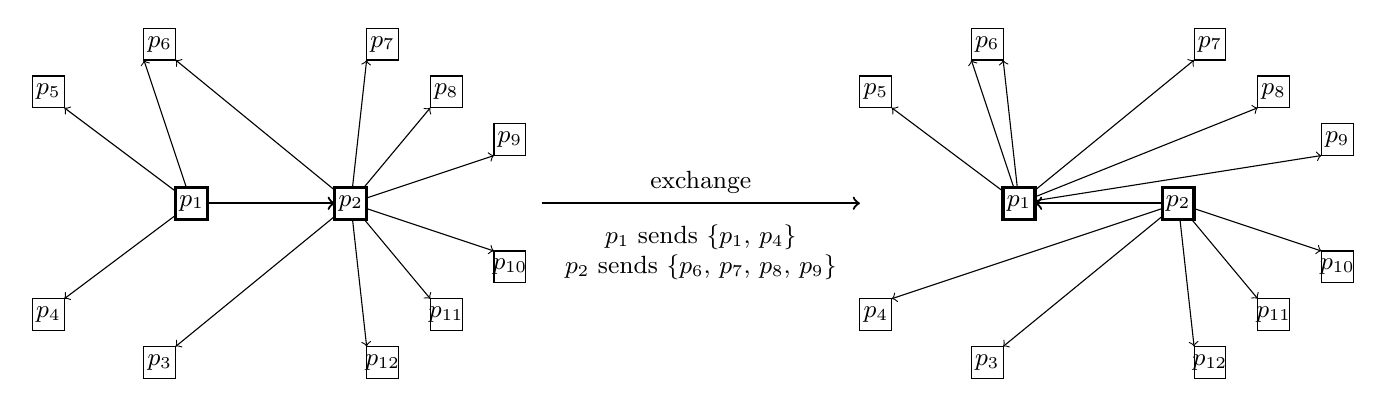
\begin{tikzpicture}[scale=1.15]
  \small

  \draw[->] (0pt,  0pt) -- ( -40pt,  30pt );
  \draw[->] (0pt,  0pt) -- ( -40pt, -30pt );
  \draw[->] (0pt,  0pt) -- ( -15pt,  45pt );

  \draw[->, thick] (0pt, 0pt) -- (45pt, 0pt);
  \draw[->] (50pt, 0pt) -- (-5pt, -45pt);
  \draw[->] (50pt, 0pt) -- (-5pt, 45pt);

  \draw[fill=white, very thick](0pt, 0pt)
  node{$p_1$}+(-5pt,-5pt)rectangle +(5pt,5pt);
  \draw[fill=white] (-10pt, 50pt)node{$p_6$} +(-5pt,-5pt) rectangle +(5pt,5pt);
  \draw[fill=white] (-45pt, 35pt)node{$p_5$} +(-5pt,-5pt) rectangle +(5pt,5pt);
  \draw[fill=white] (-45pt,-35pt)node{$p_4$} +(-5pt,-5pt) rectangle +(5pt,5pt);
  \draw[fill=white] (-10pt,-50pt)node{$p_3$} +(-5pt,-5pt) rectangle +(5pt,5pt);

  \begin{scope}[shift={(50pt,0pt)}]
  \draw[->] (0pt, 0pt) -- (   5pt, -45pt );
  \draw[->] (0pt, 0pt) -- ( 45pt, -15pt );
  \draw[->] (0pt, 0pt) -- ( 25pt, -30pt );
  \draw[->] (0pt, 0pt) -- (  25pt, 30pt );
  \draw[->] (0pt, 0pt) -- (  45pt, 15pt );
  \draw[->] (0pt, 0pt) -- (   5pt, 45pt );

  \draw[fill=white, very thick] (0pt, 0pt)
  node{$p_2$} +(-5pt,-5pt) rectangle +(5pt,5pt);
  \draw[fill=white] ( 10pt, 50pt)node{$p_{7}$}+(-5pt,-5pt)rectangle+(5pt,5pt);
  \draw[fill=white] ( 30pt, 35pt)node{$p_{8}$}+(-5pt,-5pt)rectangle+(5pt,5pt);
  \draw[fill=white] ( 50pt, 20pt)node{$p_{9}$}+(-5pt,-5pt)rectangle+(5pt,5pt);

  \draw[fill=white] ( 50pt,-20pt)node{$p_{10}$}+(-5pt,-5pt)rectangle+(5pt,5pt);
  \draw[fill=white] ( 30pt,-35pt)node{$p_{11}$}+(-5pt,-5pt)rectangle+(5pt,5pt);
  \draw[fill=white] ( 10pt,-50pt)node{$p_{12}$}+(-5pt,-5pt)rectangle+(5pt,5pt);
  \end{scope}
 

  \draw[->,thick] (110pt, 0pt) --node[anchor=south]{exchange}
  node[anchor=north, align=center]{ \ \\
    $p_1$ sends $\left\{p_1,\,p_4\right\}$\\
  $p_2$ sends $\left\{p_6,\,p_7,\,p_8,\,p_9\right\}$}
  (210pt, 0pt);

  \begin{scope}[shift={(260pt, 0pt)}]
  \draw[->] (0pt, 0pt) -- ( -40pt,  30pt );
  \draw[->] (0pt, 0pt) -- ( -15pt,  45pt );
  \draw[->] (0pt, 0pt) -- (  -5pt,  45pt );


  \draw[<-, thick] (5pt, 0pt) -- (50pt, 0pt);
  \draw[->] (50pt, 0pt) -- (-5pt, -45pt);
  \draw[->] (50pt, 0pt) -- (-40pt, -30pt);
  \draw[->] (0pt, 0pt) -- (  55pt, 45pt );
  \draw[->] (0pt, 0pt) -- ( 95pt,  15pt );
  \draw[->] (0pt, 0pt) -- ( 75pt,  30pt );

  \draw[fill=white, very thick](0pt, 0pt)
  node{$p_1$}+(-5pt,-5pt)rectangle +(5pt,5pt);
  \draw[fill=white] (-10pt, 50pt)node{$p_6$} +(-5pt,-5pt) rectangle +(5pt,5pt);
  \draw[fill=white] (-45pt, 35pt)node{$p_5$} +(-5pt,-5pt) rectangle +(5pt,5pt);
  \draw[fill=white] (-45pt,-35pt)node{$p_4$} +(-5pt,-5pt) rectangle +(5pt,5pt);
  \draw[fill=white] (-10pt,-50pt)node{$p_3$} +(-5pt,-5pt) rectangle +(5pt,5pt);

  \begin{scope}[shift={(50pt,0pt)}]
  \draw[->] (0pt, 0pt) -- (  25pt, -30pt );
  \draw[->] (0pt, 0pt) -- (  45pt, -15pt );
  \draw[->] (0pt, 0pt) -- (   5pt, -45pt );

  \draw[fill=white, very thick] (0pt, 0pt)
  node{$p_2$} +(-5pt,-5pt) rectangle +(5pt,5pt);
  \draw[fill=white] ( 10pt, 50pt)node{$p_{7}$}+(-5pt,-5pt)rectangle+(5pt,5pt);
  \draw[fill=white] ( 30pt, 35pt)node{$p_{8}$}+(-5pt,-5pt)rectangle+(5pt,5pt);
  \draw[fill=white] ( 50pt, 20pt)node{$p_{9}$}+(-5pt,-5pt)rectangle+(5pt,5pt);

  \draw[fill=white] ( 50pt,-20pt)node{$p_{10}$}+(-5pt,-5pt)rectangle+(5pt,5pt);
  \draw[fill=white] ( 30pt,-35pt)node{$p_{11}$}+(-5pt,-5pt)rectangle+(5pt,5pt);
  \draw[fill=white] ( 10pt,-50pt)node{$p_{12}$}+(-5pt,-5pt)rectangle+(5pt,5pt);
  \end{scope}

  \end{scope}
  
\end{tikzpicture}
  \caption{\label{fig:scamplonexample} Examplary exchange between two peers
    using \SCAMPLON{}. In this case, Peer $p_1$ initiates an exchange with its
    oldest neighbor $p_2$ (for simplicity sake, only the partial view of the
    peers involved in the exchange are explicitly drawn). The network on the
    left shows the network before the exchange, and the network on the right
    shows the network after the exchange. After the exchange of peers chosen at
    random, both peers $p_1$ and $p_2$ have a partial view size of $6$.}
\end{figure*}

Figure~\ref{fig:scamplonexample} (REDO EXAMPLE) depicts an exchanging procedure
between two peers $p_1$ and $p_2$. The initiating peer $p_1$ chooses its oldest
neighbor $p_2$ to perform a neighborhood exchange. The former selects
$\left\lceil{|\mathcal{P}_1|\over{2}}\right\rceil-1={4\over{2}}-1=1$ random
peer among its neighborhood, here $\left\{p_1\right\}$. To this sample, it adds
a reference to itself and sends the exchange message to $p_2$. The receipt of
the message triggers the $onExchange$ event at Peer $p_2$. Hence, the latter
chooses $\left\lceil{|\mathcal{P}_2|\over{2}}\right\rceil= {8\over{2}}=4$
random neighbors from its partial view to send back to Peer $p_1$. In this
example it chooses $\{p_6,\,p_7,\,p_8,\,p_9\}$ and sends it to
$p_1$. Afterwards, Peer $p_2$ cuts the connections to the peers it sent and
creates new one with the received peer from $p_1$. Peer $p_1$ does the same,
and additionally removes the connection chosen for the exchange, i.e., the
connection to $p_2$. Afterwards, both partial view contains $6$
neighbors. Also, we can see that $p_1$ contains two times Peer $p_6$.

\subsection{Leaving}
\label{subsec:leaving}

Using \SCAMPLON{}, the peers are free to leave the network without giving
notice. However, without any appropriate reaction, the network may collapse due
to an over zealous removal of connections. Indeed, when a peer joins the
network, it injects in it $1+ln(|\mathcal{N}|)$ connections. Nevertheless,
after few exchanges, the partial view of the joining peer becomes populated
with more neighbors. Then, if this peer leaves, it removes $ln(|\mathcal{N}|)$
connections from its partial view, and another $ln(|\mathcal{N}|)$ connections
from peers which have this peer in their partial view. Therefore, without any
crash handler, we remove $2ln(|\mathcal{N}|)$ connections instead of
$1+ln(|\mathcal{N}|)$. To alleviate this issue, each peer that detects a crash
may reestablish a connection with anyone in its neighborhood (which will
spread in the network over the exchanges). The probability of reestablishing a
connection is $1-{1\over{|\mathcal{P}|}}$. Since
${|\mathcal{P}|}\approx ln(|\mathcal{N}|)$ peers have the crashed peer in their
partial view, it is likely that all of them will reestablish a connection,
excepted one. Therefore, when a peer leaves, it approximately removes the
number of connections it injected when it joined.

\begin{algorithm}
  
\small
\SetKwProg{Function}{function}{}{}
\SetKwComment{tcp}{$\triangleright$~}{}
\DontPrintSemicolon
\LinesNumbered

\newcommand{\LET}[0]{\textbf{let}\xspace}
\newcommand{\FROM}[0]{\textup{\textbf{from}}\xspace}
\newcommand{\TO}[0]{\textup{\textbf{to}}\xspace}

\Function{\textup{onPeerDown ($q$)} \tcp*[f]{$q$: crashed/departed}} {
  \LET $occ \leftarrow 0$ \;

  \ForEach(\tcp*[f]{remove and count}) { $\langle n, age\rangle \in \mathcal{P}$ }  {
    \If {$n=q$} {
       $\mathcal{P} \leftarrow \mathcal{P}\setminus \{\langle n,\,age\rangle \}$ \;
       $occ \leftarrow occ + 1$ \;
    }
  }

  \For{$i$ \FROM $0$ \TO $occ$} {
    \tcp*[l]{probabilistically duplicates}

    \If{$\textup{rand( )}>{1\div{(|\mathcal{P}|+occ}})$} {
       \LET $\langle n,\,\_ \,\rangle \leftarrow
         \mathcal{P}[\left\lfloor \textup{rand( )}*|\mathcal{P}|\right\rfloor]$ \;
       $\mathcal{P} \leftarrow \mathcal{P} \uplus \left\{\langle n,\, 0\rangle\right\}$
    }
  }
}

\BlankLine

\Function{\textup{onArcDown($q$, $age$)} \tcp*[f]{$q$: arc arrival}} {
  $\mathcal{P} \leftarrow \mathcal{P}\setminus \{\langle q, age\rangle \}$ \;
  \tcp*[l]{systematically duplicates}
  \LET $\langle n, \_ \rangle \leftarrow
  \mathcal{P}[\left\lfloor \textup{rand( )}*|\mathcal{P}|\right\rfloor]$ \;
  $\mathcal{P} \leftarrow \mathcal{P} \uplus \left\{\langle n, 0\rangle\right\}$ \;

}

  \caption{\label{algo:unreachable}The crash handler of \SCAMPLON{}.}
\end{algorithm}

Algorithm~\ref{algo:unreachable} shows the manner in which \SCAMPLON{} deals
with crashes. When the peer $q$ is detected as crashed, a first loop counts the
occurrences of this neighbor in the partial view, and removes all of them. The,
the second loop probabilistically doubles a connection with a known peer. The
probability depends of the partial view size before the removals.

(EXAMPLE)

Note that extending the algorithms to handle three-way handshake is not
difficult: it only requires to keep track of the neighbor from where the
membership messages arrived, and forward the answer to this neighbor
accordingly. Also, there are few optimization concerning the establishments of
connections. For instance, when a peer $p$ starts an exchange with $q$, and $q$
has $p$ in its partial view, instead of inverting the link between $p$ and $q$,
and $q$ and $p$, \SCAMPLON{} does not change them. Another optimization
concerns a peer having a neighbor multiple times in its partial view. While
\SCAMPLON{} keeps such information in its partial view, only one connection per
neighbor is truly necessary.

To summarize, \SCAMPLON{} provides:
\begin{inparaenum}[(i)]
\item a logarithmically increasing partial view size compared to the global
  network size,
\item a constant complexity to establish the connections,
\item an exponentially fast convergence to a random graph.
\end{inparaenum}
Providing these three properties, \SCAMPLON{} improves the state-of-the-art
approaches~\cite{ganesh2001scamp,voulgaris2005cyclon} in the traditional
connection set-up. Furthermore, the improvement becomes crucial in the context
of three-way handshake connection set-up.  The latter becomes increasingly
important with the appearance of technologies allowing peer-to-peer within
modern web browsers.  The next section aims to demonstrate experimentally the
behavior of \SCAMPLON{}. In particular, it aims to highlight the aforementioned
properties.


%%% Local Variables:
%%% mode: latex
%%% TeX-master: "../paper"
%%% End:
